\paragraph{QuizziPedia::Front-End::Directives::TopicKeywordsDirective}

\label{QuizziPedia::Front-End::Directives::TopicKeywordsDirective}

\begin{figure}[h]
	\centering
	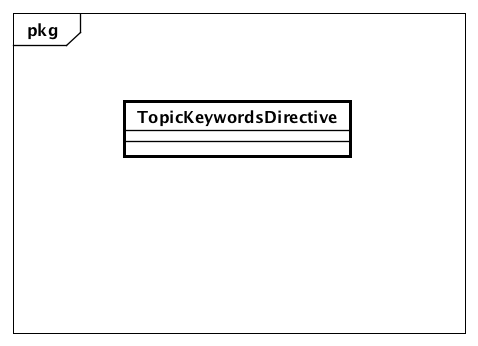
\includegraphics[scale=0.80,keepaspectratio]{UML/Classi/Front-End/QuizziPedia_Front-end_Directives_TopicKeywordsDirective.png}
	\caption{QuizziPedia::Front-End::Directives::TopicKeywordsDirective}
\end{figure}

\begin{itemize}
	\item \textbf{Descrizione}: directive che permette di gestire l'inserimento dell'argomento e delle keywords al momento della creazione della domanda;
	\item \textbf{Utilizzo}: permette l'inserimento di keywords al momento di creazione della domanda, in particolare sarà formata da:
	\begin{itemize}
		\item Un menù a tendina per selezionare l'argomento della domanda;
		\item Un campo di testo in cui inserire le keywords.
	\end{itemize}
	\item \textbf{Relazioni con altre classi}:
	\begin{itemize}
		\item \textit{IN} \texttt{TopicKeywordsController}: questa classe permette di gestire il recupero delle parole chiave di un questionario;
		\item \textit{IN} \texttt{TopicKeywordsModelView}: classe di tipo modelview la cui istanzazione è contenuta all'interno della variabile di ambiente \$scope di \textit{Angular.js\ped{G}}. All'interno di essa sono presenti le variabili e i metodi necessari per il \textit{Two-Way Data-Binding\ped{G}} tra la directive \texttt{TopicKeywordsDirective} e il controller \texttt{TopicKeywordsController};
		\item \textit{IN} \texttt{CreateQuestionnaireView}: view per la creazione del questionario; 
		\item \textit{IN} \texttt{TrueFalseQuestionsView}: view contenente i campi per creare una domanda vero/falso; 
		\item \textit{IN} \texttt{MultipleQuestionsView}: view contenente i campi per creare una domanda a risposta multipla;
		\item \textit{IN} \texttt{ConnectionQuestionsView}: view contenente i campi per creare una domanda a collegamento;
		\item \textit{IN} \texttt{ImagesSortingQuestionsView}: view contenente i campi per creare una domanda a ordinamento immagini;
		\item \textit{IN} \texttt{StringsSortingQuestionsView}: view contenente i campi per creare una domanda a ordinamento stringhe;
		\item \textit{IN} \texttt{FillingQuestionsView}: view contenente i campi per creare una domanda a riempimento testo;
		\item \textit{IN} \texttt{ClickableAreaQuestionsView}: view contenente i campi per creare una domanda ad area cliccabile;
		\item \textit{IN} \texttt{EditorQMLView}: view contenente l'editor QML per la creazione di domande personalizzate;
	\end{itemize}
	\item \textbf{Attributi}:
	\begin{itemize}
		\item \texttt{+ topics: Array} \\ Array contenente le stringhe dei nomi degli argomenti;
		\item \texttt{+ keyword: String} \\ Attributo contenente la keyword associata alla domanda/questionario;
		\item \texttt{+ controller: String} \\ Stringa contenente il nome del controller della direttiva;
		\item \texttt{+ restrict: String}: stringa che permette di definire le modalità di inserimento della direttiva all'interno della pagina;
		\item \texttt{+ scope: Scope}: oggetto scope interno della direttiva, contiene le funzionalità per gestire i dati presenti all'interno;
		\item \texttt{+ templateUrl: String}: stringa contenente il percorso del file \textit{HTML\ped{G}} che contiene la direttive.
	\end{itemize}
\end{itemize}